\documentclass[a4paper,11pt]{article}
%\usepackage[slovene]{babel}
\usepackage[utf8]{inputenc}
\usepackage[T1]{fontenc}

\usepackage{graphicx}
\usepackage{tabularx}
\usepackage{url}
\usepackage{amsmath}
\usepackage{array, multirow}
\usepackage{cprotect}

\newcolumntype{Y}{>{\centering\arraybackslash}X}

\begin{document}
\thispagestyle{empty}
%\setlength{\parindent}{0em}


\includegraphics[scale=0.35]{UUlogo.png}

\vspace{50mm}

\begin{center}
\begin{large}
Data Mining: Assignment 2 \\[3mm]
\textbf{
\uppercase{Text Classification for the Detection of Opinion Spam}} \\[25mm]
\end{large}

\begin{tabularx}{\textwidth}{YY}
Ana Borovac & Argyro (Iro) Sfoungari \\
6584446 & 6528015
\end{tabularx}
\end{center}

\vfill

October, 2018

\newpage

\tableofcontents

\vspace{2.5cm}

\begin{abstract}
Our task was to compare different classifiers (Naive Bayes, Logistic regression, Classification tree, Random forests), which predict if a hotel review is deceptive or truthful. We trained our models on 640 negative reviews of hotels in Chicago area; half of them were deceptive and half of them were truthful reviews. Furthermore, we analysed the effect of hyperparameters, e.~g.\ coplexity parameter for pruning the Classification tree. We concluded....
\end{abstract}

\newpage

\section{Introduction}
Nowadays email filters are able to classify spam and not spam emails quite successfully. Imagine now that you have a web site with hotel reviews and your goal is to offer the most truthful reviews but you can not check every single review and it is also hard to recognise when the review is not truthful. Therefore you would like to have a mechanism which is going to help you to achieve your goal. 

In this assignment we tried to solve the above problem with 4 methods; Naive Bayes, logistic regression, classification tree and random forests. Before we started, we analysed the work that has been done already (section \ref{sec: relatedwork}). Next, we did some data preprocessing, it is described in the section \ref{sec: data}. Used methods are explained in the section \ref{sec: methods} and analysis of the results (section \ref{sec: results}) is in the section \ref{sec: analysis}.

\section{Related work}
\label{sec: relatedwork}
The authors of “Finding Deceptive Opinion Spam by Any Stretch of the Imagination” \cite{article1} compared truthful and deceptive positive reviews for hotels. They used Naive Bayes and Support Vectors Machine classifiers. For comparison they also had 3 human untrained judges which tried to predict if a review was real or fake.  The results had shown that automated classifiers outperform human judges in almost every metric (precision, recall, F-score). They explain that with that untrained humans often focus on unreliable cues to
deception. One of the results was also that models trained only on unigrams outperformed all non--text-categorizations approaches (genre identification and psycholingustic deception detection). Furthermore, the results were even better when bigrams were used.

In the article “Negative Deceptive Opinion Spam” \cite{article2} the authors created corpus of gold standard 400 reviews on 20 Chicago hotels and then used them to compare $n$-gram--based Support Vector Machine classifiers with untrained human judges. They concluded that the best detection performance was achived through automated classifiers. 

\section{Data}
\label{sec: data}
Our data consisted of 400 negative deceptive and 400 negative truthful hotel reviews that have been collected by Myble Ott and others (\cite{article2}, \cite{article1}). 

\subsection{Data preprocessing}
Before modeling we did some data preprocessing in order to get better models for predicting if a review is fake or real. First step in data preprocessing was to remove punctuation marks, after that we made every letter lower case, we also removed stopwords, numbers and excess whitespace. 

Next, we created a test and a training set. Because we wanted to use cross validation, we divided our data into 5 folds (each of size 160 samples - 80 fake reviews and 80 truthful reviews). So, 4 of the folds represented a training set, the remaining 5th fold was a test set. 

At that moment every unique word from the training reviews was a feature.  A number of features was large therefore we removed the words as features which occur less than 1~\% of training documents.

After that we created a new training set which consisted all the features from the previous training set and bigrams. We again removed bigrams that occur in lass that  3~\% of training documents. At the end we had two training sets ready to be used. 

How we chose the percentage of the features which were used is more detailed explained in the subsection \ref{subsec: naiveBayes}.

\section{Methods}
\label{sec: methods}

We used different classifiers to model our task:
\begin{itemize}
	\item Naive Bayes (generative linear classifier); Naive Bayes is a probabilistic classifier. Class is predicted from features which has highest probability with independence assumption (features are independent within each class) \cite{naiveBayes}:
\[
\hat{c} = \arg\max_{c \in C} P(c) \prod_{i = 1}^m P(x_i | c)
\] 
	\item Logistic regression (discriminative linear classifier); Logistic regression is one of discriminative classification methods \cite{logisticRegression}. That means that modelling of probability, how likely are we to predict a class $c$ with given input, is direct. In a binary case we predict class $1$ if it holds:
\[
\frac{P(Y = 1 | x)}{P(Y = 0 | x)} > 1; \quad P (Y = 1 | x) = \frac{1}{1 + e^{-\beta^T x}}
\]
otherwise we predict class $0$.
	\item Classification tree (flexible classifier); Classification trees are usually not the best models \cite{classificationTrees}, but are easy to interpret and can handle both numerical and categorical attributes. 
	\item Random forests (flexible classifier); Random forests are improved classification trees, where the best split is chosen among $k$ random features and not among all of them \cite{randomForestsL}. 
\end{itemize}

\section{Results}
\label{sec: results}

After the preprocessing procedure, we started analysing the data based on the aforementioned classifiers. Initially, we will present you the data analysis step by step, as we worked during the assignment.

\subsection{Naive Bayes}
\label{subsec: naiveBayes}

Initially we started with the Naive Bayes classifier trained with the code from the lectures \cite{code}. We considered that it would be useful to create several combinations of unigrams and bigrams by changing the appearance rate of the terms, in order to receive the highest accuracy percentage. Although in the beginning we considered that the highest percentage was achieved by removing the terms that occur less than 1~\% for unigrams and less than 35~\% for bigrams (table \ref{tab: naiveBayes}), later we realised that this combination did not involve any bigrams at all. So we had to continue our research by choosing a different combination of percentages, in order to include results for bigrams as well and draw to specific conclusions. The percentage we finally chose was 99~\% for unigrams and 97~\% for bigrams.

\begin{table}[h!]
\centering
\begin{tabular}{c | c || c | c}
\multicolumn{2}{c||}{$_{\text{Terms presence}}$ \textbackslash $^{\text{Accuracy}}$} & Unigrams & Bigrams \\ \hline \hline
\multirow{7}{*}{99~\%} & 99~\% & 0{,}87 & 0{,}53 \\ \cline{2-4}
& 97~\% & 0{,}85 & 0{,}49 \\ \cline{2-4}
& 80~\% & 0{,}84 & 0{,}63 \\ \cline{2-4}
& 76~\% & 0{,}87 & 0{,}77 \\ \cline{2-4}
& 70~\% & 0{,}87 & 0{,}87 \\ \cline{2-4}
& 68~\% & 0{,}86 & 0{,}86 \\ \cline{2-4}
& 65~\% & \textbf{0{,}87} & \textbf{0{,}87} \\ \hline
95~\% & 65~\% & 0{,}84 & 0{,}84 \\ \hline
80~\% & 70~\% & 0{,}67 & 0{,}67 \\ \hline
\multirow{2}{*}{70~\%} & 80~\% & 0{,}60 & 0.5 \\ \cline{2-4}
& 70~\% & 0{,}60 & 0{,}60 \\ 
\end{tabular}
\caption{First two columns represent terms presence; in how many training documents did a specific unigram or bigram appeared. Last two columns show accuracies of Naive Bayes classifiers trained on the selected features.}
\label{tab: naiveBayes}
\end{table}

For the other classifiers, we tried to compare the accuracy not only using their pure forms but also changing the hyper parametric values to compare the differences for unigrams and bigrams. 

\subsection{Classification tree}

For Classification trees we followed the following process: we used the \verb|rpart| library of R \cite{rpart} in order to grow a tree and then the function \verb|prune|, in order to prune it. Initially we used the complexity parameter equals to  $0{,}037$ but afterwards we used the \verb|plotcp| function in order to find the optimal value for the complexity parameter. The function uses cross-validation after which the results are represented in a plot.

Following the graph (figure \ref{fig: cp}), we tested different values for the complexity parameters, some of them are presented in the table \ref{tab: classificationTree}. 

\begin{figure}[h!]
\centering
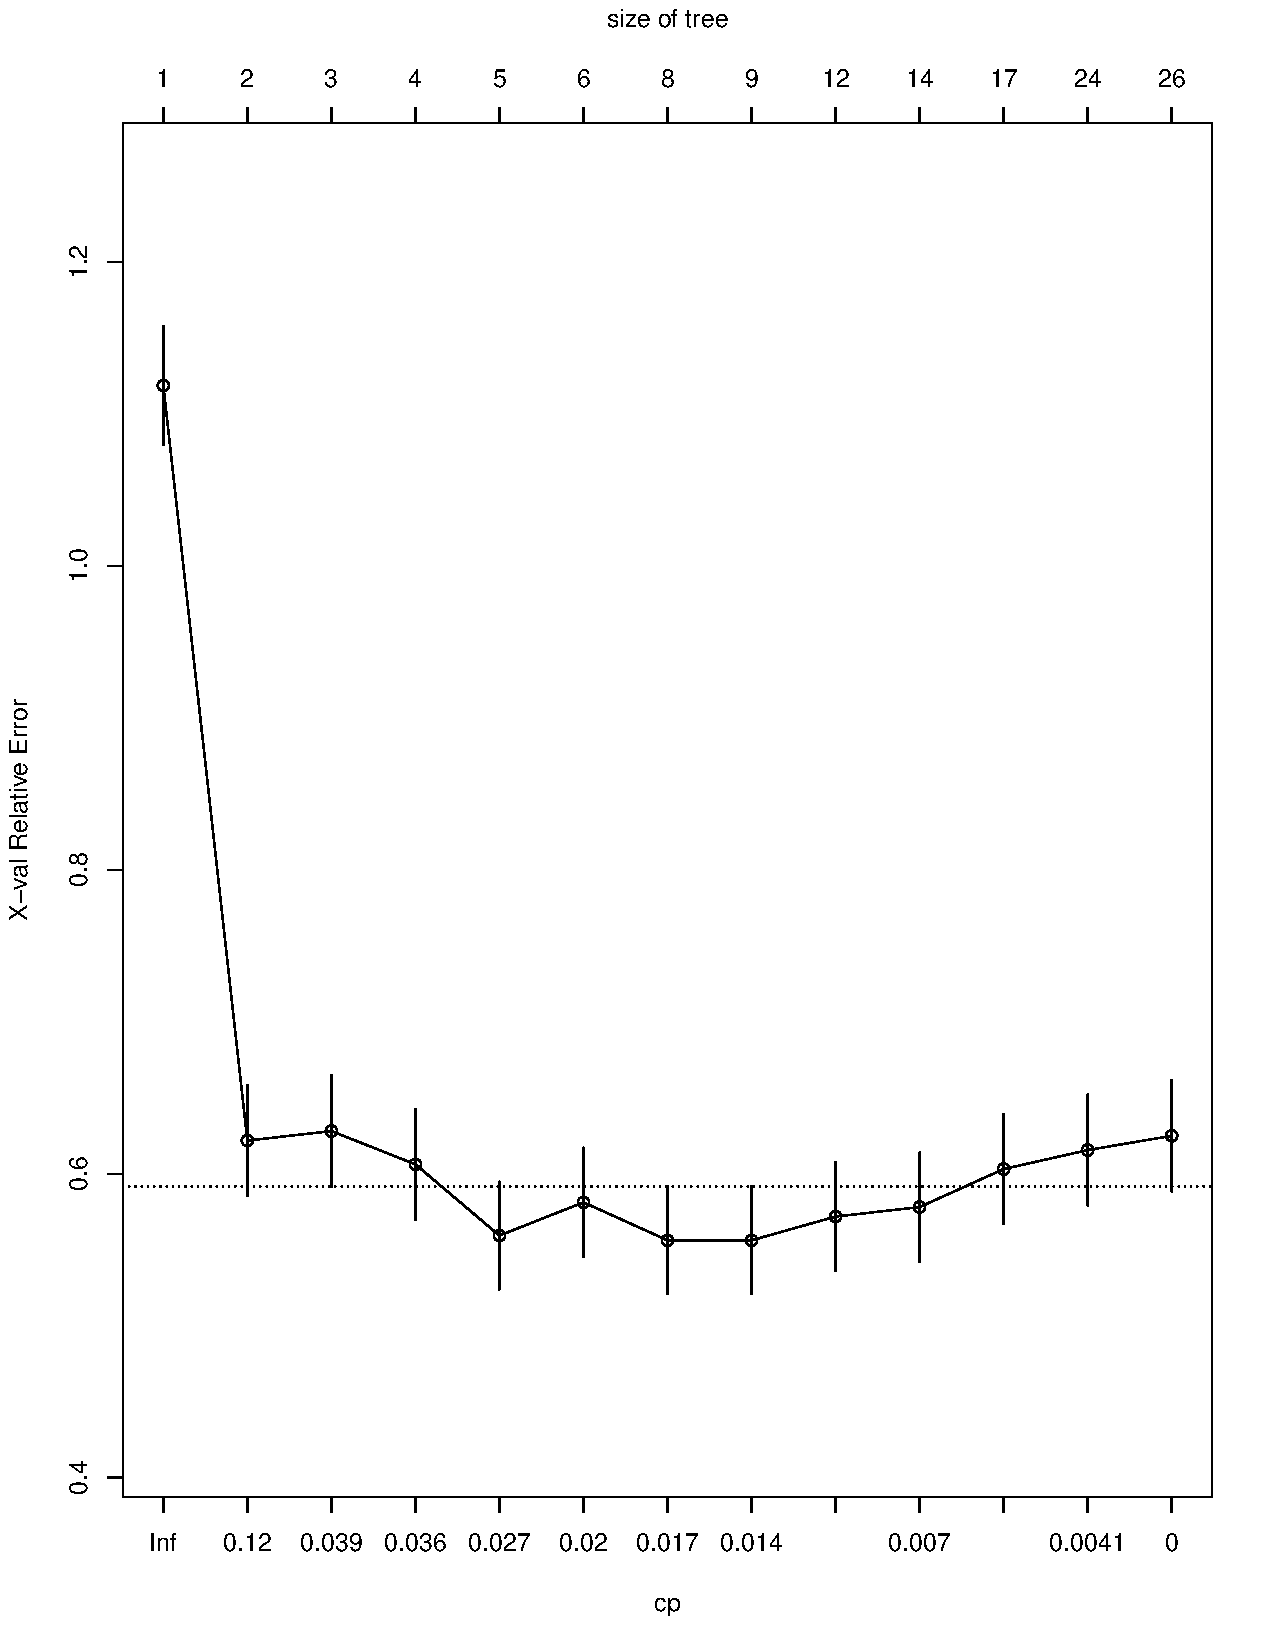
\includegraphics[width = 0.66\textwidth]{CP.pdf}
\cprotect\caption{Plot returned from a function \verb|plotcp|, which gives a visual representation of the cross-validation results in a Classification tree.}
\label{fig: cp}
\end{figure}

\begin{table}[h!]
\centering
\begin{tabular}{m{5cm} @{,} l || c | c}
\multicolumn{2}{c ||}{$_{\text{Complexity parameter}}$ \textbackslash $^{\text{Accuracy}}$} & Unigrams & Bigrams \\ \hline \hline
\multicolumn{1}{r @{,}}{$\qquad \qquad\ $ 0} & 12 & \textbf{0{,}70} & \textbf{0{,}70} \\ \hline
\multicolumn{1}{r @{,}}{0} & 037 & 0{,}68 & 0{,}68 \\ \hline
\multicolumn{1}{r @{,}}{0} & 027 & 0{,}69 & 0{,}69 \\ \hline
\multicolumn{1}{r @{,}}{0} & 007 & 0{,}68 & 0{,}67 \\ \hline
\multicolumn{1}{r @{,}}{0} & 00041 & 0{,}68 & 0{,}68 
\end{tabular}
\caption{Accuracies from Classification trees pruned with the complexity parameter from first column.}
\label{tab: classificationTree}
\end{table}

As it can be seen clearly from the table, the optimal value for the complexity parameter is $0{,}12$ as it gives the highest accuracy. At this point we noted that for both cases the accuracy remains the same. So we concluded that bigrams do not contribute to classification trees.

\subsection{Random Forests}

For random forests we worked as follows. We used the function \verb|randomForest| (from R libraby verb|randomForest| \cite{randomForestsL}) and we implemented various tests, changing the number of trees (\verb|ntree|) and the number of variables randomly sampled as candidates at each split (\verb|mtry|). 

\begin{table}[h!]
\centering
\begin{tabular}{m{2cm} |c || c | c}
\multicolumn{2}{c||}{$_{\text{Number of trees, mtry}}$ \textbackslash $^{\text{Accuracy}}$} & Unigrams & Bigrams \\ \hline \hline
$\quad\ \ $ 100 & 4 & 0{,}75 & 0{,}42 \\ \hline
\multirow{3}{*}{$\quad\ \ $ 200} & 4 & 0{,}77 & 0{,}39 \\ \cline{2-4}
& 6 & \textbf{0{,}82} & \textbf{0{,}44} \\ \cline{2-4}
& 8 & 0{,}81 & 0{,}45 \\ \hline
\multirow{3}{*}{$\quad\ \ $ 300} & 4 & 0{,}79 & 0{,}43 \\ \cline{2-4}
& 6 & 0{,}80 & 0{,}45 \\ \cline{2-4}
& 8 & 0{,}80 & 0{,}44 \\ 
\end{tabular}
\caption{First column presents the number of trees in a Random forest, second column is the numbers of features selected in each step of the algorithm and the last two columns represent calculated accuracies.}
\label{tab: randomForests}
\end{table}

From the table \ref{tab: randomForests} we came to the conclusion that the best combination is achieved by 200 trees and mtry equals to 6, while accuracy levels for bigrams are very low.

\begin{table}[h!]
\centering
\begin{tabular}{c || c | c}
$_{\text{Lambda}}$ \textbackslash $^{\text{Accuracy}}$ & Unigrams & Bigrams \\ \hline \hline
lambda.1se & 0{,}80 & 0{,}78 \\ \hline
lambda.min & \textbf{0{,}81} & \textbf{0{,}82} 
\end{tabular}
\caption{Accuracies for two different Logistic regression models; one with largest value of lambda which is 1 standard error apart from minimum, and the minimum lambda.}
\label{tab: logisticRegression}
\end{table}

\subsection{Logistic regression}

For logistic regression model we used \verb|cv.glmnet| function from \verb|glmnet| library \cite{glmnet}. The function does $k$-fold cross-validation and as a result returns a value for \verb|lambda|. We left the default value of $k$, which is set to $10$. Since we know that our model is binomial (\verb|family = “binomial”|), we were able to set $\verb|type.measure|$ to “class”. This means that the loss which is used for cross-validation is misclassification error. We tried to make some tests changing the value of the user-supplied lambda sequence (table \ref{tab: logisticRegression}). \\

Accuracy, Precision, Recall and F1\_score with (99~\% of unigrams, 97~\% of bigrams, number of trees = 200, \verb|mtry| = 6, lambda.1se and \verb|cp| = 0{,}12) for 8 models are represented in the table \ref{tab: results}.

\begin{table}[h!]
\centering
\begin{tabular}{l | l || c | c | c | c} 
\multicolumn{2}{c|}{} & $\quad$A$\quad$ & $\quad$P$\quad$ & $\quad$R$\quad$ & $\quad$F1$\quad$ \\ \hline \hline
\multirow{2}{*}{Naive Bayes} & Unigrams & 0{,}81 & 0{,}82 & 0{,}80 & 0{,}80 \\ \cline{2-6}
& Bigrams & 0{,}47 & 0{,}40 & 0{,}71 & 0{,}52 \\ \hline
\multirow{2}{*}{Classification Trees} & Unigrams & 0{,}71 & 0{,}61 & 0{,}65 & 0{,}63 \\ \cline{2-6}
& Bigrams & 0{,}71 & 0{,}61 & 0{,}65 & 0{,}63 \\ \hline
\multirow{2}{*}{Random Forests} & Unigrams & 0{,}81 & 0{,}85 & 0{,}74 & 0{,}77 \\ \cline{2-6}
& Bigrams & 0{,}47 & 0{,}70 & 0{,}93 & 0{,}49 \\ \hline
\multirow{2}{*}{Logistic Regression} & Unigrams & 0{,}79 & 0{,}67 & 0{,}81 & 0{,}73 \\ \cline{2-6}
& Bigrams & 0{,}79 & 0{,}66 & 0{,}84 & 0{,}74
\end{tabular}
\caption{Accuracies (A), Precisions (P), Recalls (R) and F1\_scores (F1) for 8 models.}
\label{tab: results}
\end{table}


\section{Analysis}
\label{sec: analysis}

After studying the results in the section \ref{sec: results}, we have concluded to some specific assumption which we will present you below. Initially, it would be beneficial to compare the generative linear model (Naive Bayes) with the discriminative linear model (Logistic regression). As it is clear from the tables, Naive Bayes gives a slightly higher accuracy when it comes to unigrams, therefore we can talk about a negligible difference. However, when we include bigrams in our analysis, the discriminative linear model seems to be much more efficient and accurate than Naive Bayes as the difference is enormous. Then we compared the discriminative linear model with Random forests. Once again the precision percentage is almost the same for the two classifiers, or it may become a bit higher for Random forests if we change the hyperparameters properly (number of trees, randomly selected features) for unigrams. Concerning the bigrams Logistic regression is repeatedly the best choice, as it gives by far the highest accuracy, while on the contrary Random forests give the lowest. As it mentioned earlier (Naive Bayes classifier case), the highest accuracy was achieved without the existence of bigrams, so we could say that bigrams do not contribute in performance improvement.

Regarding the most important terms towards truthful or deceptive reviews, in order to receive some accurate results we used the \verb|importance| function, this function extracts the important measures produced by \verb|randomForest|.

We ran the code twice. Once setting the \verb|class| parameter equals to 0 (deceptive) and another one setting \verb|class| equals 1 (truthful). Consequently we receive as the most important terms for fake reviews
the following: 
\begin{enumerate}
	\item Chicago, 
	\item location, 
	\item seemed, 
	\item hotel.chicago,
	\item luxury. 
\end{enumerate}
Concerning the genuine reviews the most important terms presented in priority order are: 
\begin{enumerate}
	\item Chicago, 
	\item location, 
	\item luxury, 
	\item rude, 
	\item seemed.
\end{enumerate}

\bibliographystyle{plain}
\bibliography{references}

\end{document}










